\chapter{Figuras}

\vspace*{-3in}

\begin{figure}
\vspace{2.4in}
\caption{Ejemplo de computaci\'on \textit{REST} sem\'antica.}
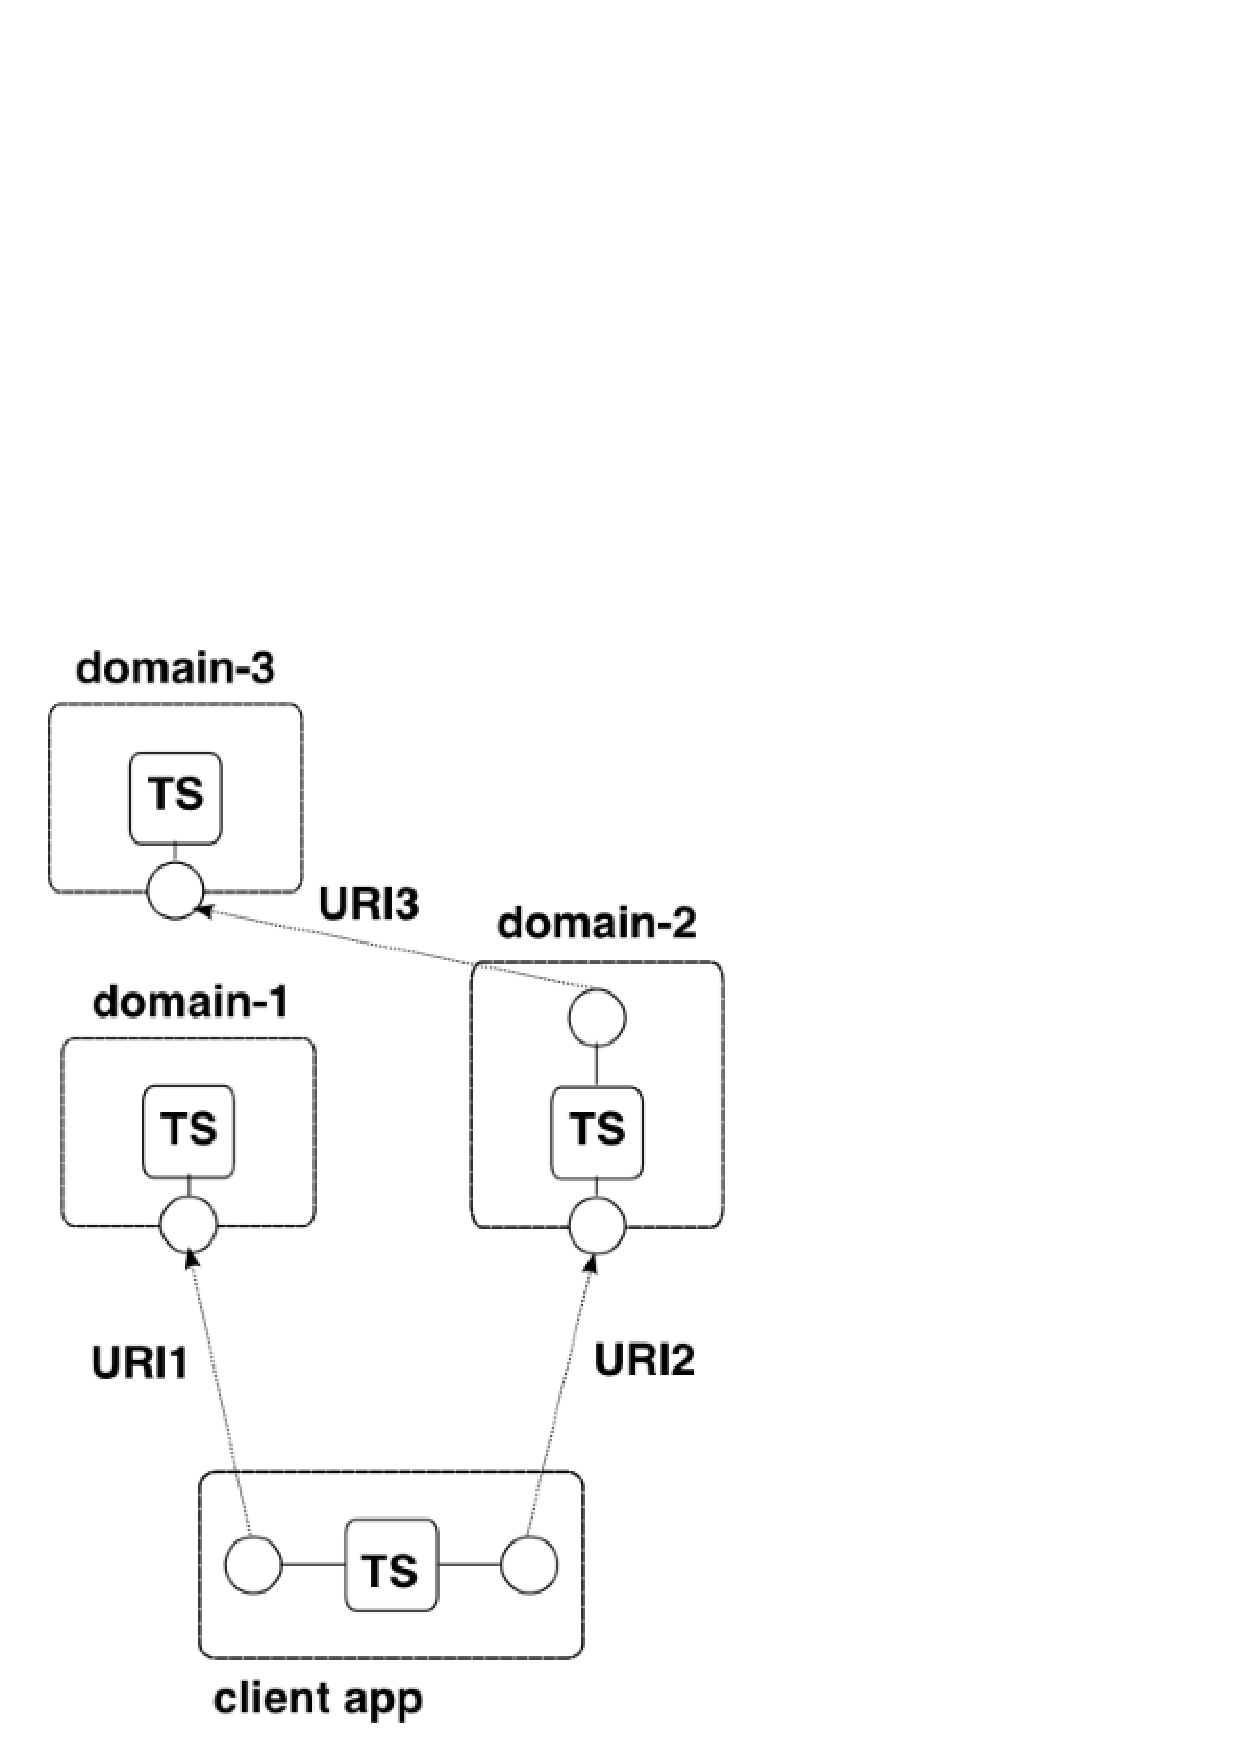
\includegraphics[width=0.5\textwidth]{figura1}
\label{figura1}
\end{figure}

\clearpage
\newpage

\vspace*{-3in}

\begin{figure}
\vspace{2.4in}
\caption{Diferentes transformaciones codificadas en un documento \textit{R2RML}}
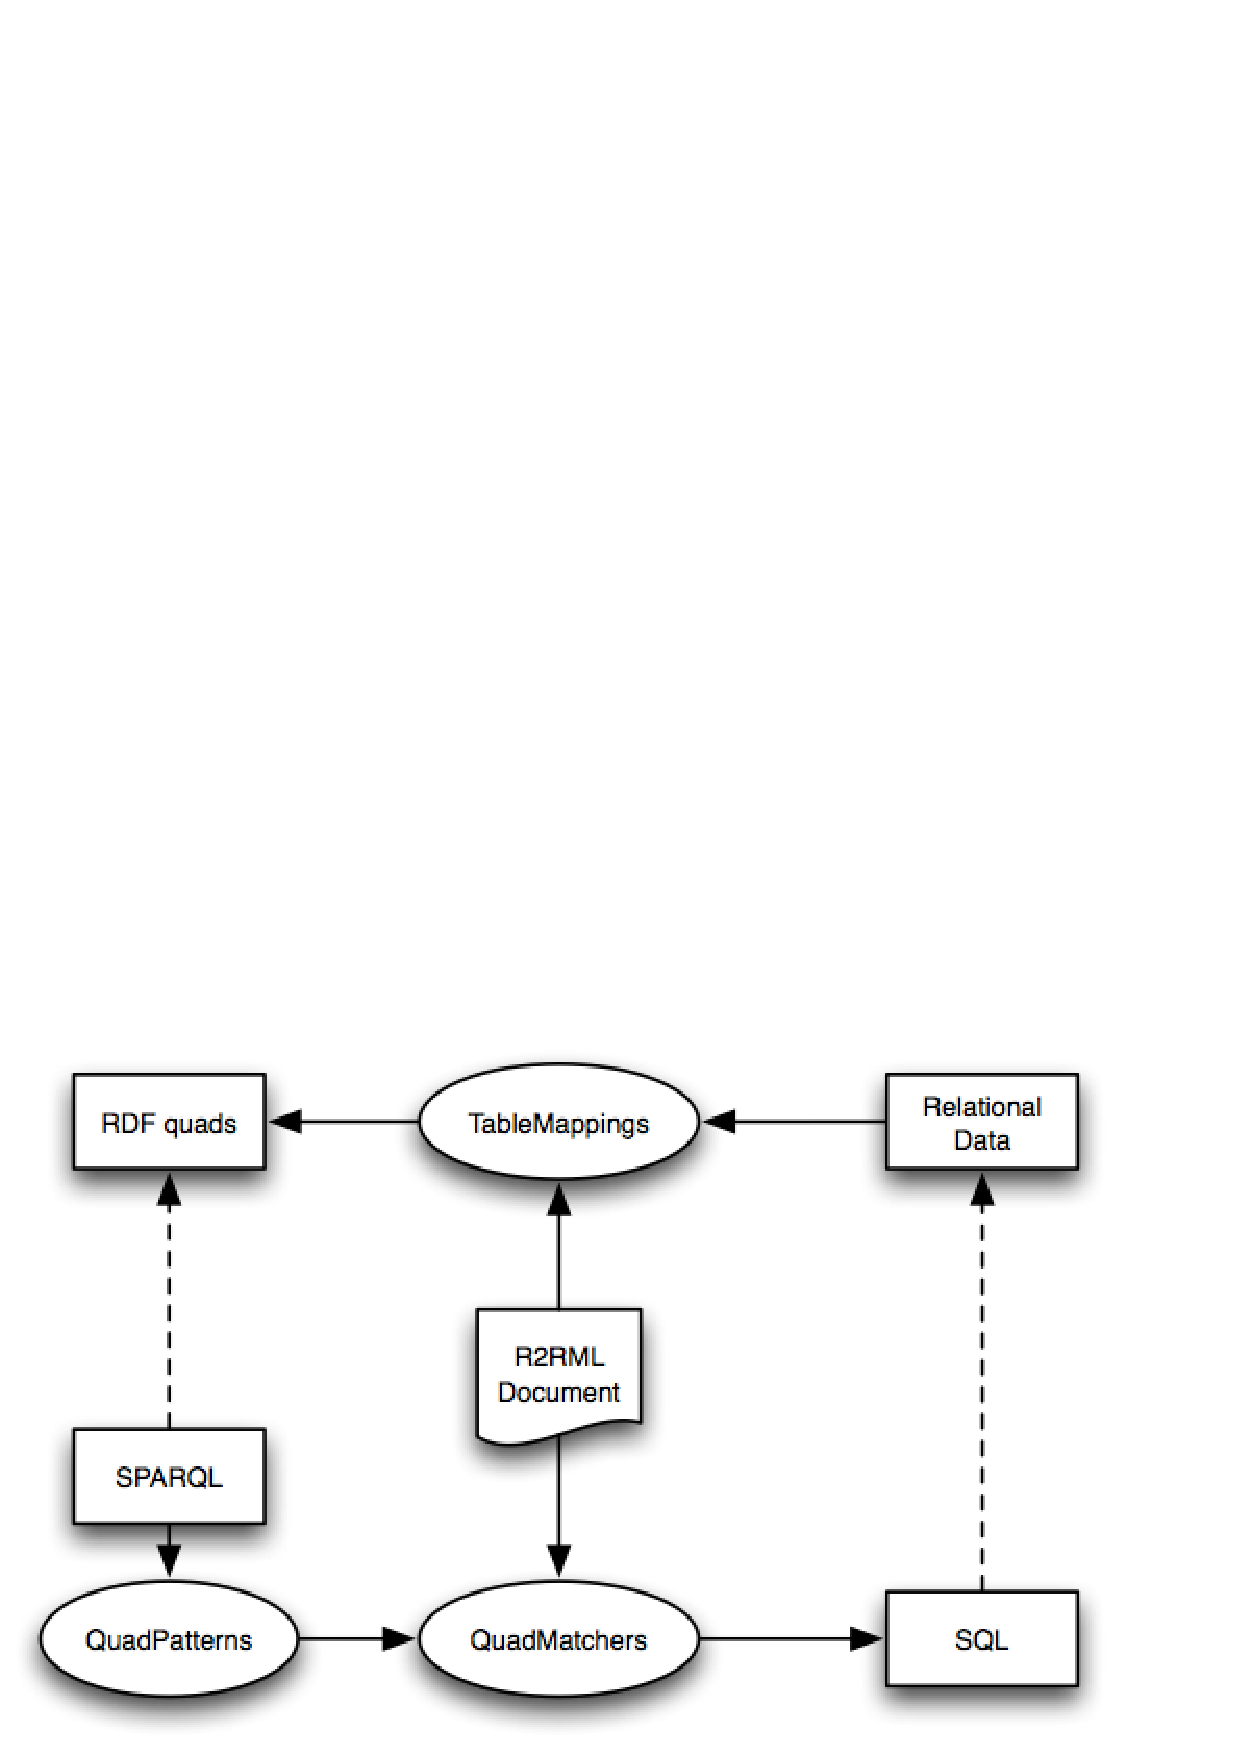
\includegraphics[width=0.5\textwidth]{figura2}
\label{figura2}
\end{figure}

\clearpage
\newpage

\vspace*{-3in}

\begin{figure}
\vspace{2.4in}
\caption{Inserci\'on de dos \textit{quads}}
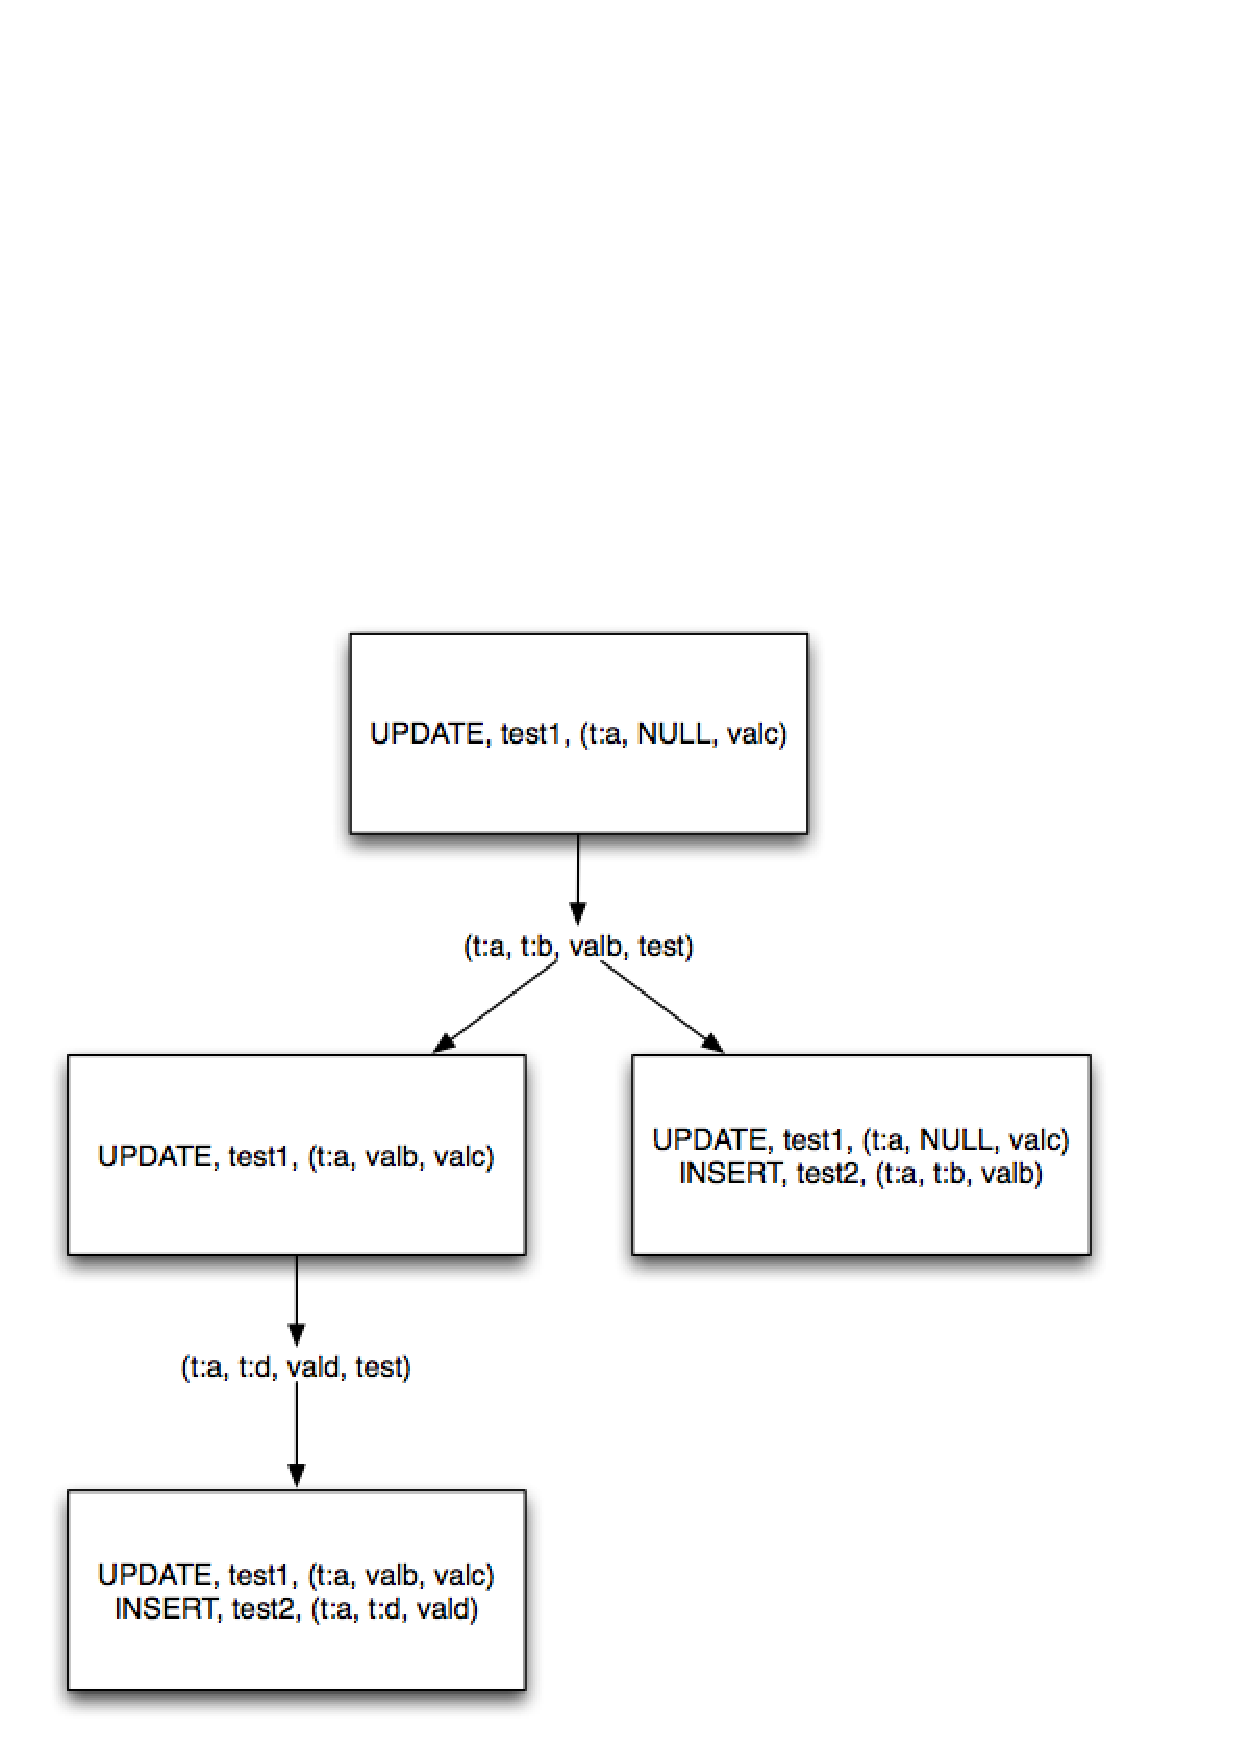
\includegraphics[width=0.5\textwidth]{figura3}
\label{figura3}
\end{figure}

\clearpage
\newpage

\vspace*{-3in}

\begin{figure}
\vspace{2.4in}
\caption{Principales componentes del repositorio \textit{RDF}.}
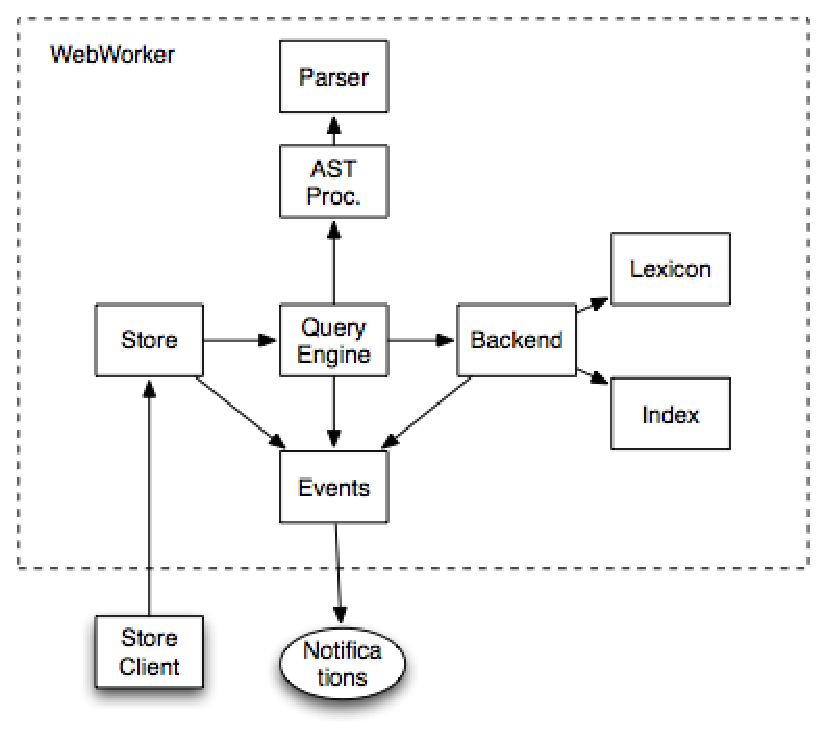
\includegraphics[width=0.5\textwidth]{figura4}
\label{figura4}
\end{figure}

\clearpage
\newpage

\vspace*{-3in}

\begin{figure}
\vspace{2.4in}
\caption{Flujo de informaci\'on en el sistema.}
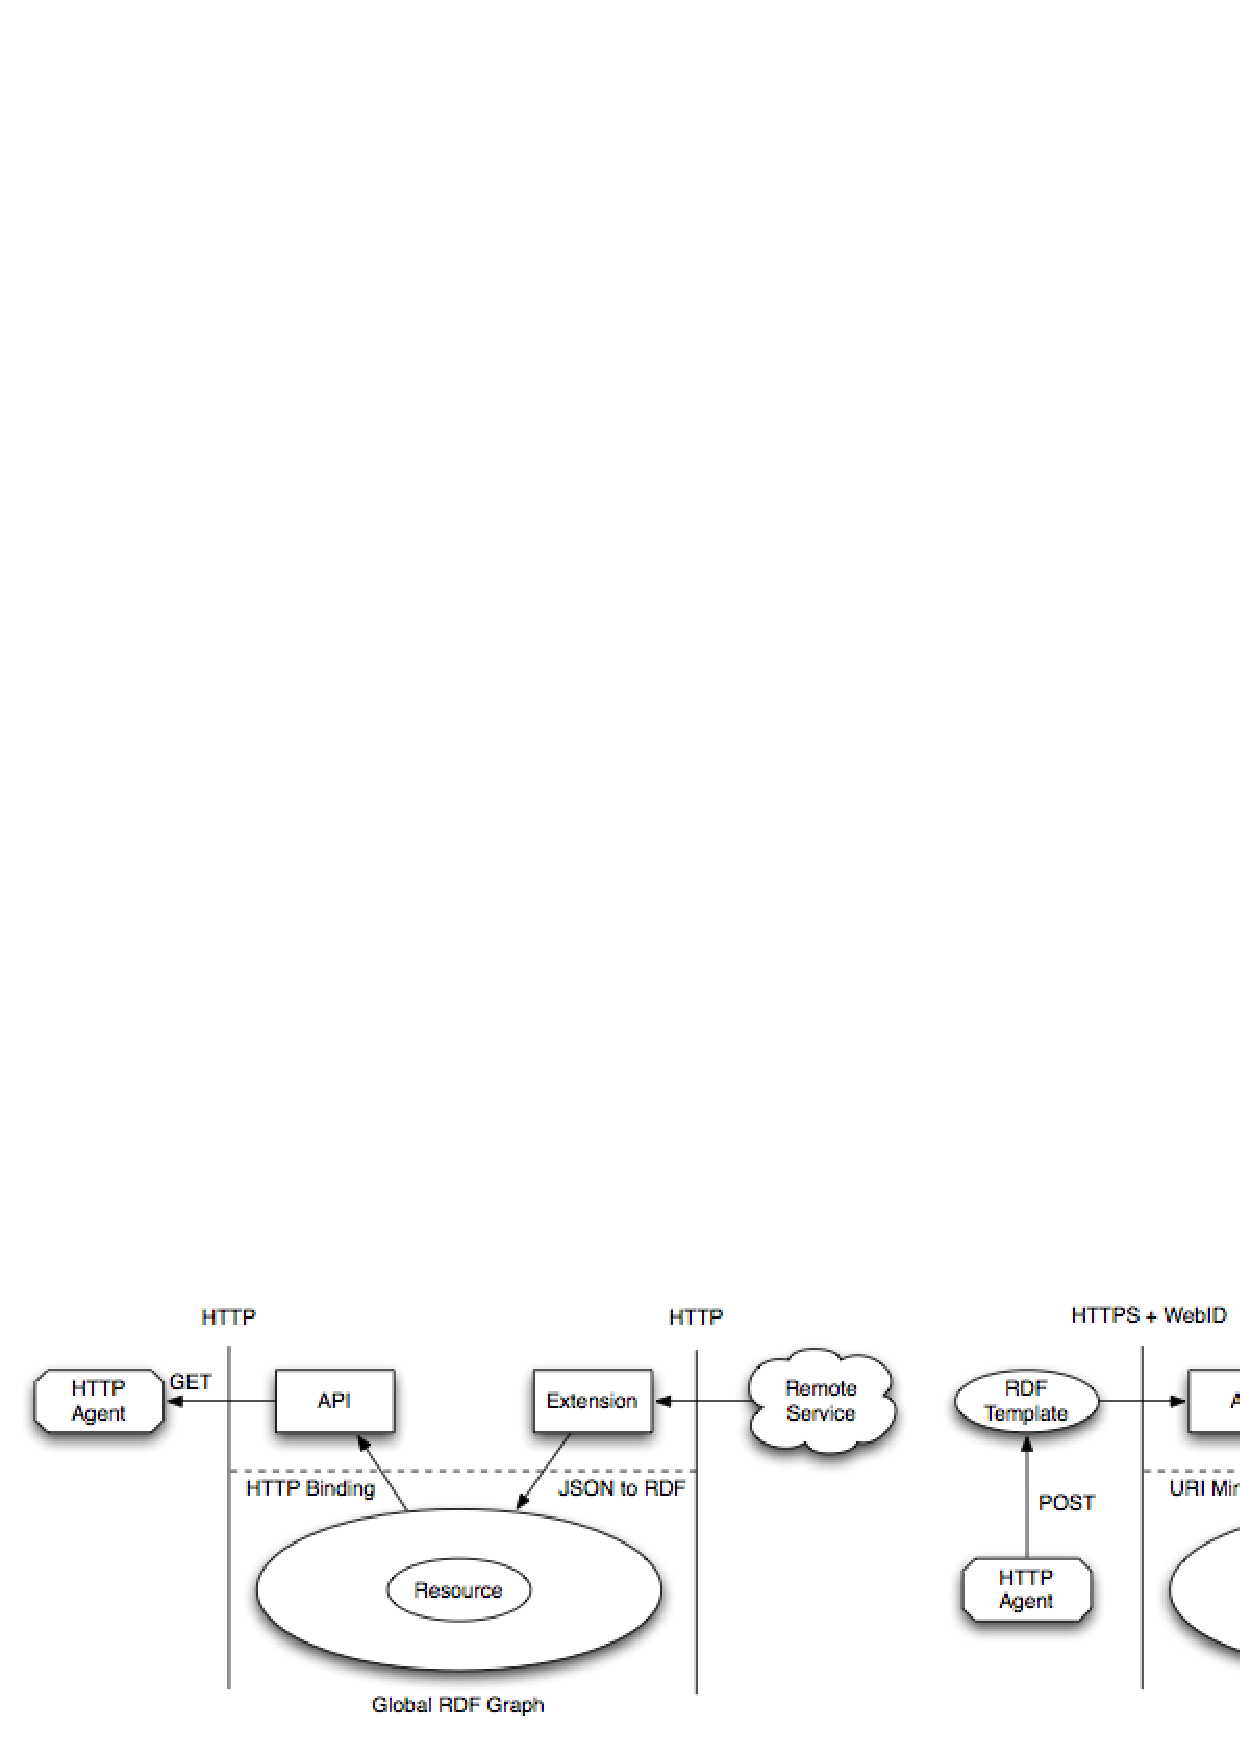
\includegraphics[width=0.5\textwidth]{figura5}
\label{figura5}
\end{figure}

\clearpage
\newpage


\vspace*{-3in}

\begin{figure}
\vspace{2.4in}
\caption{Aplicaci\'on \textit{JavaScript} mostrando el flujo de actividad de un usuario.}
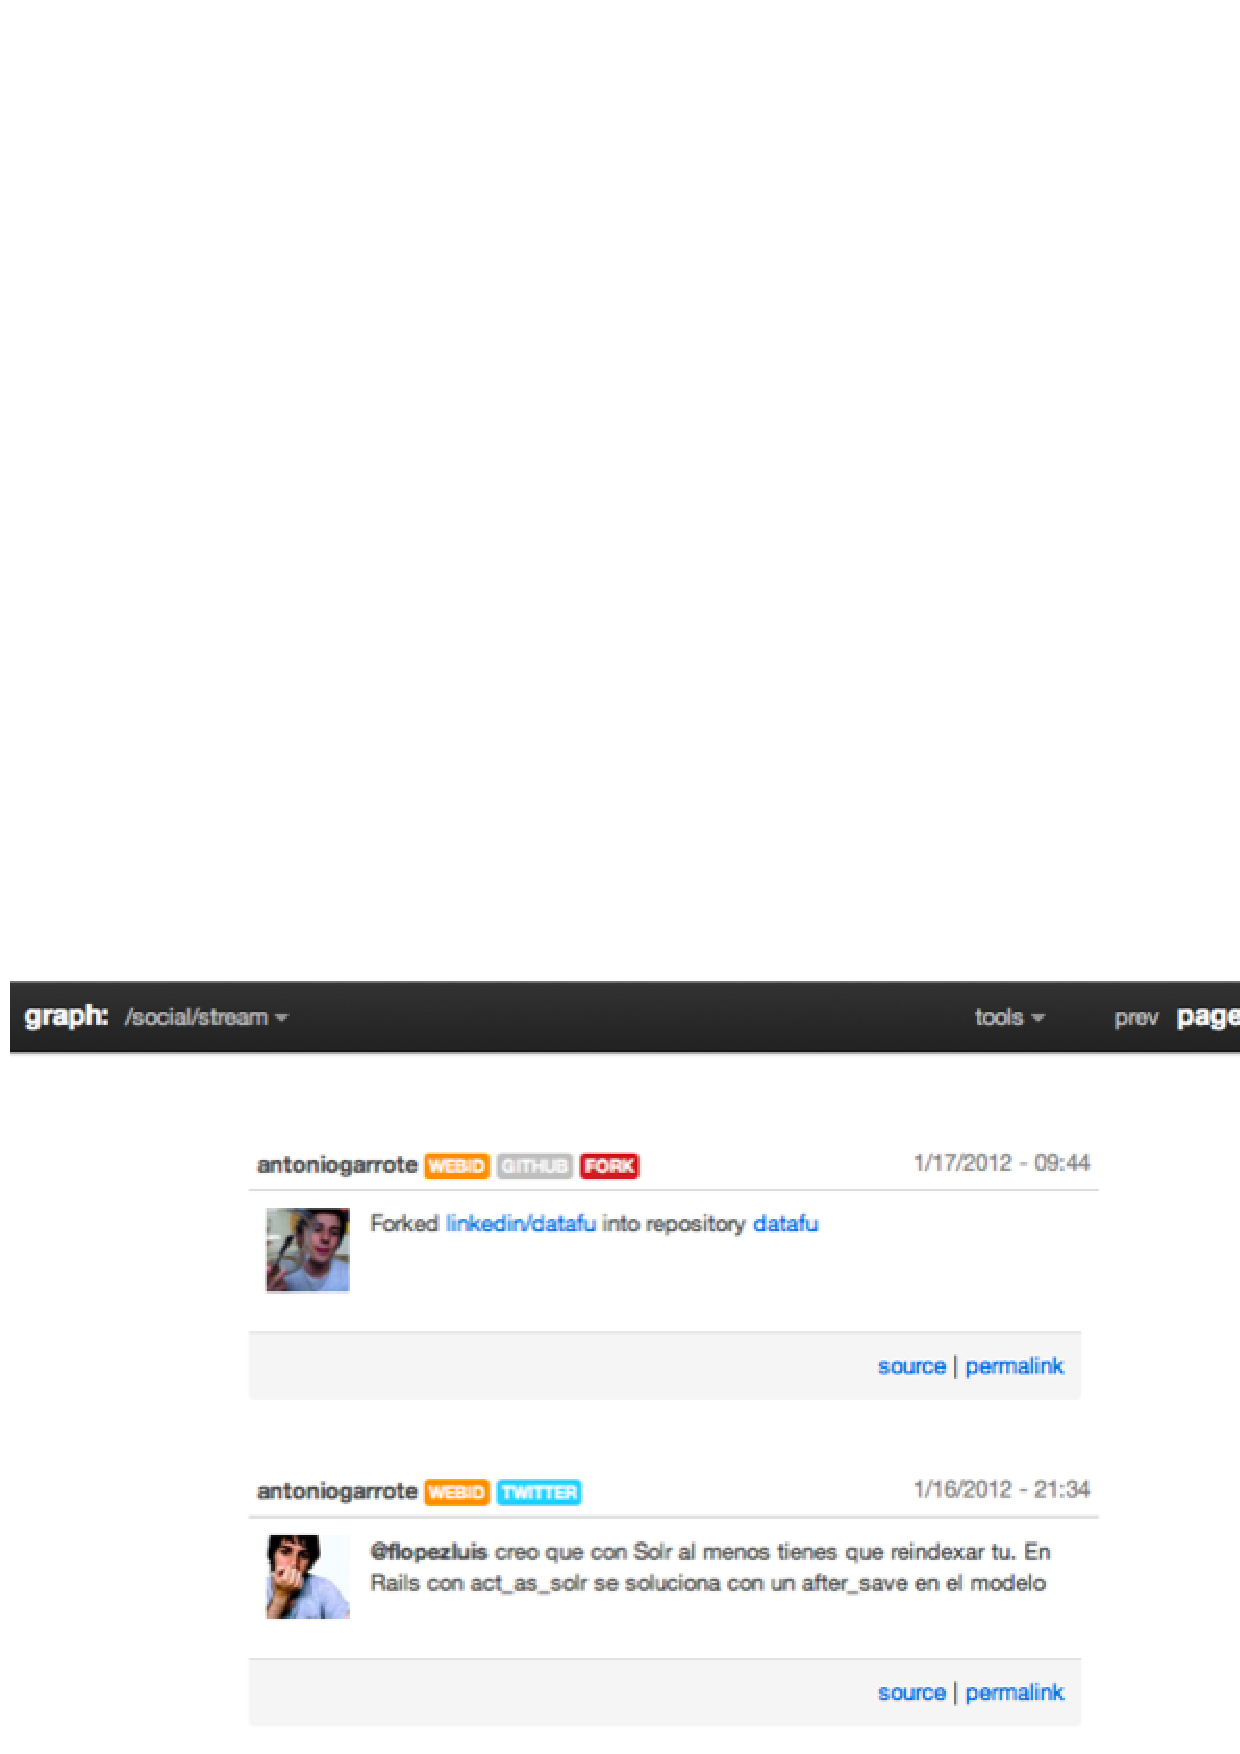
\includegraphics[width=0.5\textwidth]{figura6}
\label{figura6}
\end{figure}

\clearpage
\newpage


\vspace*{-3in}

\begin{figure}
\vspace{2.4in}
\caption{Visualizaci\'on generada por la biblioteca a partir del c\'odigo de la tabla \ref{tabla13}}
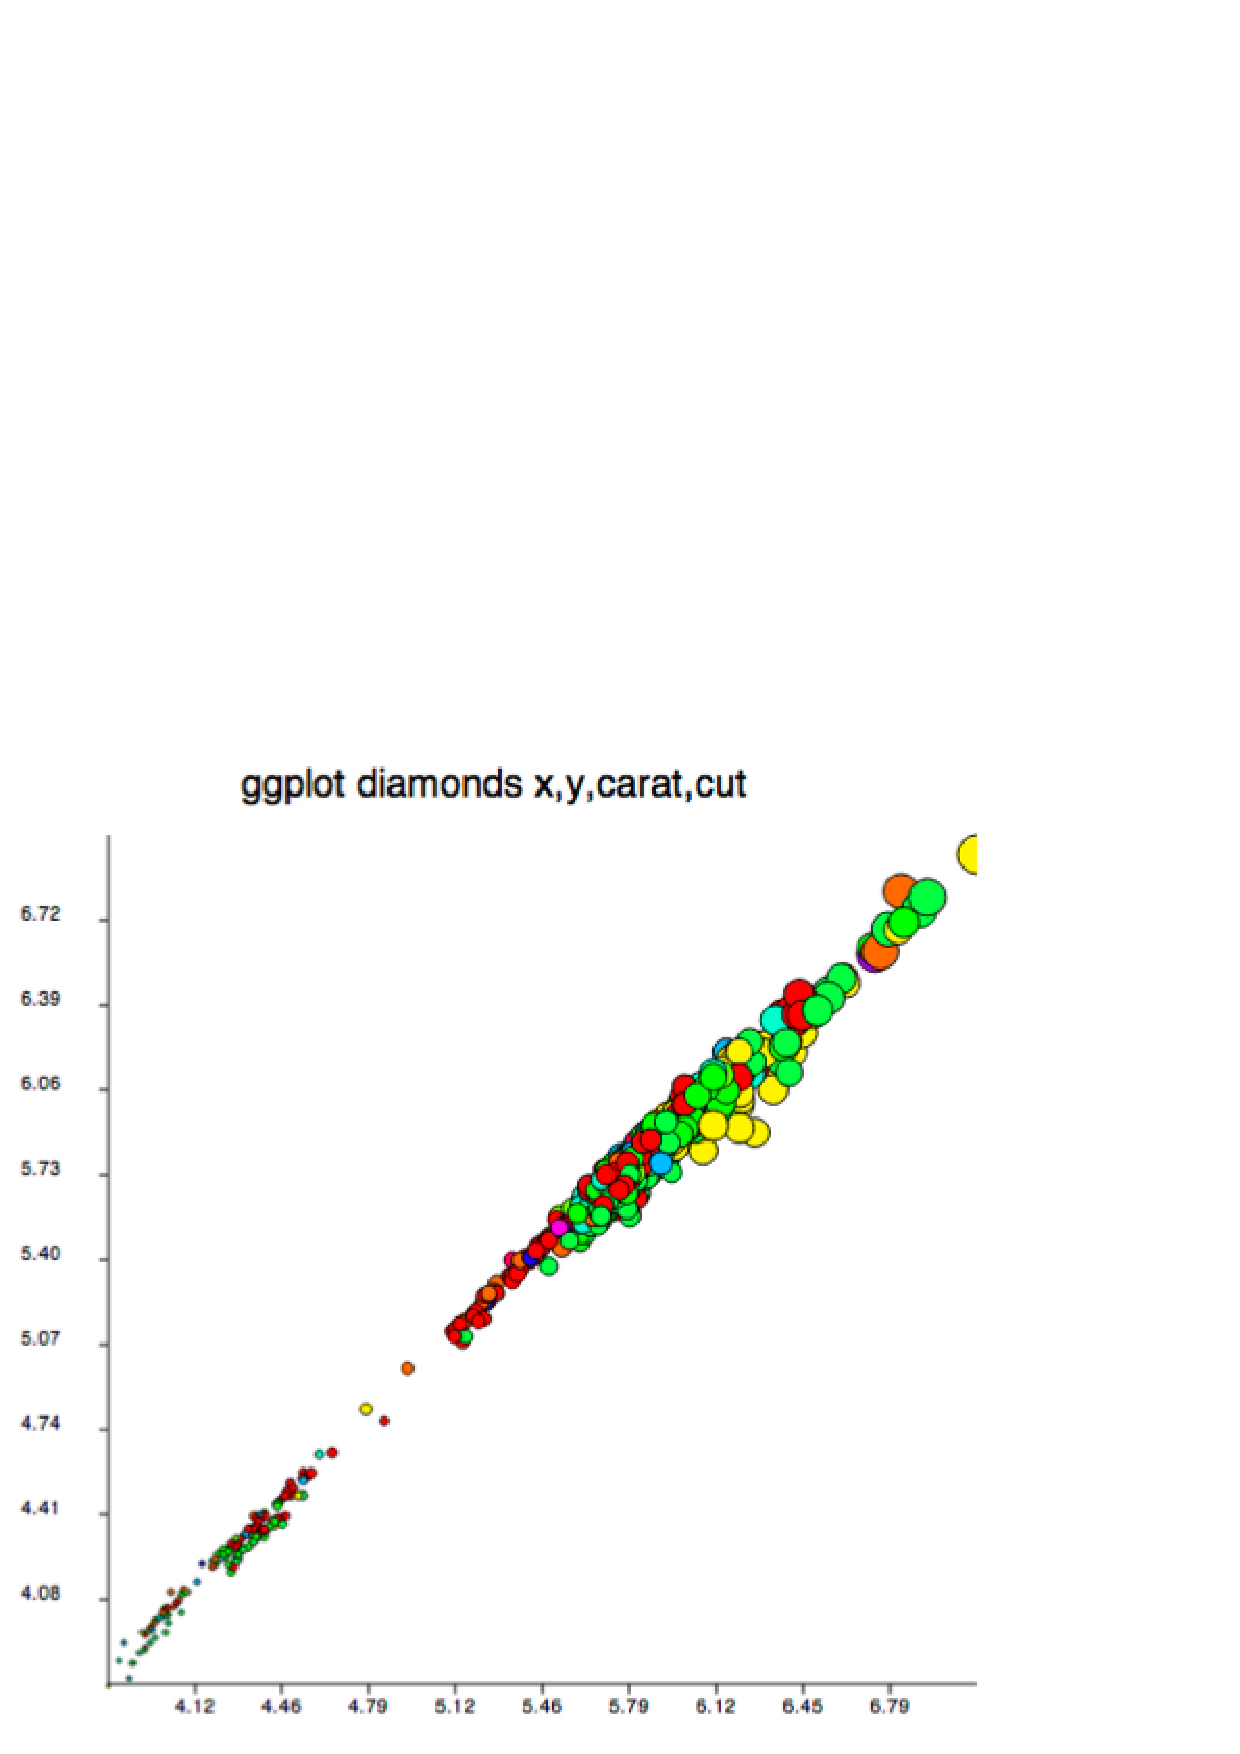
\includegraphics[width=0.5\textwidth]{figura7}
\label{figura7}
\end{figure}

\clearpage
\newpage
